% \begin{frame}
%   \frametitle{What this talk is about}
%   \begin{center}
%     \emph{Handlers for \alert<1->{algebraic effects} provide a compelling alternative to \alert<1->{monads} as a basis for \alert<1->{effectful programming}.}
%   \end{center}
% \begin{itemize}
%   \item \textbf{Key idea:} Separate effect signatures from their implementation.
%   \item \textbf{Consequent:} High-degree of modularity.
% \end{itemize}
% {\footnotesize{Definitions will follow later\dots}}
% \end{frame}

\section{PART 1: The problem}

\begin{frame}
  \frametitle{Programs are inherently effectful}
  Programs may\dots
  \begin{itemize}
    \item \dots halt prematurely
    \item \dots diverge
    \item \dots be stateful (e.g. modify a global state)
    \item \dots communicate via a network
    \item \dots print to standard out
  \end{itemize}
  A pure\footnote{By pure we mean a program that has no effects.} program is not much fun.
\end{frame}

% \begin{frame}
%   \frametitle{Fundamental different approaches to effects}
%   \begin{description}
%     \item[\alert<1->{Imperative}] Repeatedly performs implicit effects on shared global state.
%     \item[\alert<1->{Functional}] Encapsulates effects in a computational context.
%   \end{description}
%   \uncover<2->{This talk is oriented around \emph{functional} programming with effects.}
% \end{frame}

\begin{frame}
  \frametitle{Function signatures (I)}
  \begin{align*}
    f : \mathbb{Z} \to \mathbb{Z} && \text{Mathematical pure function}\\
    \text{int } f(\text{int } x)   && \text{C/C++ (impure) function}\\
    f : \text{int} \to \text{int} && \text{ML (impure) function}
  \end{align*}
\end{frame}

\begin{frame}
  \frametitle{Let's be explicit about effects}
  \begin{block}{Effect annotation}
    An effect annotation gives a static description of the potential run-time behaviour of a computation.
  \end{block}
  Benefits
  \begin{itemize}
    \item Serves as documentation (clarity)
    \item Compiler can apply specific optimisations
    \item Possible to reason more precisely about programs
  \end{itemize}
\end{frame}

\begin{frame}
  \frametitle{Enter the Monad}
  \begin{center}
    %``\textit{Shall I be pure or impure?}''
    ``Have you considered using a monad?''
    \begin{figure}
      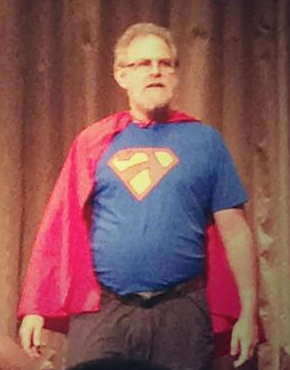
\includegraphics[scale=0.3]{figures/lambdaman.png}
      \caption{Philip Wadler aka. Lambda Man}
    \end{figure}
  \end{center}
\begin{itemize}
  \item The Essence of Functional Programming (1992)
  \item The Marriage of Effects and Monads (with Peter Thiemann, 2003)
\end{itemize}
\end{frame}

\begin{frame}
  \frametitle{Function signatures (II)}
  \begin{align*}
    &f : \mathbb{Z} \to \mathbb{Z}  && \text{Mathematical pure function}\\
    &\text{int } f(\text{int } x)   && \text{C/C++ (impure) function}\\
    &f : \text{int} \to \text{int}  && \text{ML (impure) function}\\
    \hline
    &f :: \text{Int} \to \text{IO Int} && \text{Haskell effect annotation}\\
    &\uncover<3->{\text{int } f(\text{int } x)\; \text{throws IOException} && \text{Java effect annotation}}\\
    &\uncover<4->{f : (\text{Int}) \xrightarrow{\{Read:\text{String},Write:\text{String}\to ()\}\,} \text{Int} && \text{Links effect annotation}}
  \end{align*}
\end{frame}

% \begin{frame}
%   \frametitle{Monads}
%   \begin{definition}
%     A monad is a triple $(m, return, bind)$ where
%     \begin{itemize}
%       \item $m$ is a type constructor
%       \item $return : a \to m\, a$
%       \item $bind   : m\, a \to (a \to m\, b) \to m\, b$
%     \end{itemize}
%   \end{definition}
% \end{frame}

% \begin{frame}
%   \frametitle{Great! Many monads, many effects}
%   A couple of monads and their ``effect interpretation''
%   \begin{description}
%     \item[\alert<1->{IO $a$}] May perform I/O, returns $a$
%     \item[\alert<1->{Reader $r$ $a$}] May read from $r$, returns $a$
%     \item[\alert<1->{Writer $w$ $a$}] May write to $w$, returns $a$
%     \item[\alert<1->{State $s$ $a$}] May read/write some state $s$, returns $a$
%     \item[\alert<1->{Maybe $a$}] May fail, returns $a$ on success
%   \end{description}
%   Sadly, monads do not compose well.
% \end{frame}